\documentclass[sigconf]{acmart}

\usepackage{booktabs} % For formal tables
\usepackage[ansinew]{inputenc}
\usepackage{amsmath,amsthm,amssymb,latexsym,amsfonts}
\usepackage{graphicx}
\usepackage{algorithm}
\usepackage[noend]{algpseudocode}

% Copyright
%\setcopyright{none}
%\setcopyright{acmcopyright}
%\setcopyright{acmlicensed}
\setcopyright{rightsretained}
%\setcopyright{usgov}
%\setcopyright{usgovmixed}
%\setcopyright{cagov}
%\setcopyright{cagovmixed}
\makeatletter
\def\BState{\State\hskip-\ALG@thistlm}
\makeatother

% DOI
% \acmDOI{10.475/123_4}

% ISBN
% \acmISBN{123-4567-24-567/08/06}

%Conference
\acmConference[CS 651]{Course Project}
\acmYear{2018 Winter}
\copyrightyear{2018}


% \acmArticle{4}
% \acmPrice{15.00}

% These commands are optional
%\acmBooktitle{Transactions of the ACM Woodstock conference}
\editor{Jimmy Lin}


\begin{document}
\title{Logistic Regression for Sentiment Analysis on Large Scale Social Media Posts via Apache Spark}


\author{Peng Shi}
\affiliation{%
  \institution{University of Waterloo}
}
\email{peng.shi@uwaterloo.ca}

\author{Wei Yang}
\affiliation{%
  \institution{University of Waterloo}
}
\email{w85yang@uwaterloo.ca}

\author{Masijia Qiu}
\affiliation{%
  \institution{University of Waterloo}
}
\email{m23qiu@uwaterloo.ca}

% The default list of authors is too long for headers.
% \renewcommand{\shortauthors}{Peng et al.}



\begin{abstract}

The project presents simple distributed implementations of logistic regression (LR) with several variants, including Gradient Descent (GD) based, Stochastic Gradient Descent (SGD) based and Mini-batch Stochastic Gradient Descent (MBSGD) based ones. These implementations are tested on the sentiment analysis tasks, where detailed hyper-parameters analysis is provided. 

\end{abstract}
%
% The code below should be generated by the tool at
% http://dl.acm.org/ccs.cfm
% Please copy and paste the code instead of the example below.
%
\begin{CCSXML}
<ccs2012>
 <concept>
  <concept_id>10010520.10010553.10010562</concept_id>
  <concept_desc>Computer systems organization~Embedded systems</concept_desc>
  <concept_significance>500</concept_significance>
 </concept>
 <concept>
  <concept_id>10010520.10010575.10010755</concept_id>
  <concept_desc>Computer systems organization~Redundancy</concept_desc>
  <concept_significance>300</concept_significance>
 </concept>
 <concept>
  <concept_id>10010520.10010553.10010554</concept_id>
  <concept_desc>Computer systems organization~Robotics</concept_desc>
  <concept_significance>100</concept_significance>
 </concept>
 <concept>
  <concept_id>10003033.10003083.10003095</concept_id>
  <concept_desc>Networks~Network reliability</concept_desc>
  <concept_significance>100</concept_significance>
 </concept>
</ccs2012>
\end{CCSXML}


\keywords{Logistics regression, gradient decent, sentiment analysis}

\maketitle

\section{Introduction}
\label{sec:introduction}

Logistic Regression (LR) is a widespread and useful machine learning algorithm in academia and industrial for its simplicity and effectiveness. However, as the data is inflating rapidly, these machine learning algorithms and tools are needed to be adapted to fit the big-data era. MapReduce \cite{dean2008mapreduce} is a popular algorithm in distributed computing area while Hadoop \cite{shvachko2010hadoop} and Spark \cite{zaharia2010spark} are two open-source framework for large-scale data processing. 

Today, big data community and machine learning community have sharply developed and several machine learning frameworks for distributed computing have emerged, including MLLib, Mahout and RHadoop \cite{witten2016data}. However, for newbie to this area, these mature but complicated machine learning libraries are hard due to the compact code structure and they have no idea of how to "get the hand dirty". 

In this paper, we provide simple but comprehensive implementations for logistic regression and its variants including different optimization methods and regularization. These implementations provide the beginners a good chance to learn the basic concepts of logistic regression and its spark implementation. Furthermore, they can learn how to modify these simple code to enhance the implementation and even provide more functions. 

In this paper, we have following contributions:

We offer several simple implementations for logistic regression and its variants. These implementations could be a guidance of distributed computing and machine learning. 

We create a large tweets sentiment dataset with four-byte hashing feature, which can be used for further experiments.

We provide rigorous hyper-parameter analysis for three variants of logistic regression implementations.

\section{Background and Related Work}
\label{sec:relatedWork}

Let's start with an overview of machine learning. Given $X$ to be the input space while $Y$ the output space, the set of training samples $D = \big\{ (x_1, y_1), (x_2, y_2)...(x_n, y_n) \big\} $ from the $X$ x $Y$ space, naming the labeled examples. Usually, $x_i$ represents a featured vector where $x_i \in \mathbf{R}^d$. In supervised classification task, $y_i$ comes from a finite set. when in the binary classification, $y \in \big\{ -1, +1\big\} $. A function $f$: $X \Rightarrow Y$ describing the data characteristics is introduced in the supervised machine learning tasks. The optimized case will minimize the "loss" function $L$ that quantifiably measures the discrepancy between predicted $f(x_i)$ and the actual result $y_i$. Minimizing the quantity $\sum_{(x_i, y_i) \in D} L(f(x_i), y_i)$, the best $f$ in the learned model is selected from a hypothesis space. Then it can be employed on previously unknown data to make predictions or offer predictive analysis. \cite{christopher2016pattern} \cite{franklin2005elements} Dealing with a two-class problem as the tweets sentiment, we apply the binary logistic regression to assign observations onto  two classes. 

Three components are of the most significance in the machine learning solutions: the data, the features extracted from the data, and the model. Among them, the size of the dataset is dominant given the accumulated real-world experience over the last decades. \cite{halevy2009unreasonable} \cite{lin2010data} Simple models on massive data perform better than sophisticated modes on small data. \cite{banko2001scaling} \cite{brants2007large}

The traditional machine learning assumed sequential algorithms on data fit in memory, which is no more realistic in the information bang era. Multi-core \cite{chu2007map} and cluster-based solutions \cite{agarwal2014reliable} offer new opportunities. Techniques occurs for example learning decision trees and the ensembles \cite{svore2011large}, MaxEnt models \cite{mcdonald2009efficient}, structured perceptrons \cite{mcdonald2010distributed} and so on. These approaches work well when 'data is king' for their ability to process massive amount of data. Despite the gaining popularization of large-scale learning, few published studies focus on machine learning \textit{workflows} and how such tools integrate with data management platforms. Google detects adversarial advertisements on Sculley et al. \cite{sculley2011detecting} Facebook builds its data platform on Hive. \cite{thusoo2010hive} Cohen et al. applies the integration of predictive analysis into traditional RDBMSes \cite{cohen2009mad}. 

\section{Base Algorithm}
\subsection{Logistic Regression}
\label{subsection:logistic}

Logistic regression \cite{harrell2001ordinal} transforms its output using the logistic sigmoid function to return a probability value which can then be mapped to two or more discrete classes. Assuming a two-class problem with a training set $D = \big\{ (x_1, y_1), (x_2, y_2)...(x_n, y_n) \big\} $, where $x_i$ are feature vectors and $y_i \in \big\{ -1, +1 \big\}$, a class of linear discriminative functions can be defined of the form:

\begin{equation}
F(x): \mathbf{R}^N \rightarrow \big\{ -1, +1 \big\}
\end{equation}

\begin{equation}
F(x) = \begin{cases}
    +1 \quad if \ w \cdot x \geq t \\
    -1 \quad if \ w \cdot x < t 
    \end{cases}
\end{equation}

where $t$ represents a decision threshold and $w$ is the weight vector. The modeling process usually optimizes the weight vector based on the training data $D$, and the decision threshold is subsequently tuned by various operational constraints. To learn $w$, lots of methods have been proposed to optimize different forms of loss functions or objective functions defined over the training data, where logistic regression is one particularly well-established technique interpreting the linear function $w \cdot x$ as the logarithmic odds of $x$ belonging to class +1 over -1, i.e., 

\begin{equation}
log[\frac{p(y=+1|x)}{p(y=-1|x)}] = w \cdot x
\end{equation}

The objective of regularized logistic regression (using Gaussian smoothing) is to identify the parameter vector $w$ that maximizes the conditional posterior of the data.

\begin{equation}
L = exp(-\lambda w^2 /2) \cdot \prod_i p( y_i | x_i )
\end{equation}

where 

\begin{equation}
p(y=+1|x)= \frac{1}{(1+exp(-w \cdot x))}
\end{equation}

and

\begin{equation}
\begin{split}
p(y=-1|x) &= 1-p(y=+1|x) \\
  &=\frac{1}{(1+exp(w \cdot x))}.
\end{split}
\end{equation}

In this project, three type of the variants are applied accordingly: Gradient Descent (GD) based, Stochastic Gradient Descent (SGD) based and Mini-batch Stochastic Gradient Descent (MBSGD) based.

\subsection{Gradient Descent}
\label{subsection:logisticGD}

Recall the basic Gradient Descent method, it is accomplished by adjusting the weight vector in the direction opposite to the gradient of log( $L$ ):

\begin{equation}
\begin{split}
-\bigtriangledown log(L) &= \lambda w + \sum_i \frac{1}{p(y_i |x_i )} \frac{ \vartheta}{\vartheta w} p(y_i |x_i )  \\
  &=\lambda w + \sum_i y_i p(y_i |x_i )(1-p(y_i |x_i ))
\end{split}
\end{equation}

\subsection{Stochastic Gradient Descent}
\label{subsection:logisticSGD}

While in GD the whole training set is considered before taking one model parameters update step, in SGD only one data point is considered for each model parameters update step, cycling over the Training Set. \cite{bottou2010large} In SGD update, the gradient is computed based on a single training instance, the update to the weight vector upon seeing the $i$th training example is given by 

\begin{equation}
w \leftarrow w + \eta \cdot [ - \lambda w + y_i \cdot p( y_i | x_i )(1-p( y_i | x_i ))]
\end{equation}

Noted that each element in the weight vector is decayed at each iteration. However, when the feature vectors of training instances are very sparse (as is true for our project), we can simply delay the updates for features until they are actually seen. 

\subsection{Mini-Batch Stochastic Gradient Descent}
\label{subsection:logisticMBSGD}

Mini-Batch Stochastic Gradient Descent (MBSGD) \cite{ioffe2015batch} is a variation of the gradient descent algorithm that splits the training dataset into small batches that are used to calculate model error and update model coefficients. It chooses to sum the gradient over the mini-batch or take the average of the gradient which further reduces the variance of the gradient. Mini-batch gradient descent seeks to find a balance between the robustness of stochastic gradient descent and the efficiency of batch gradient descent. It is the most common implementation of gradient descent used in the field of deep learning.

\subsection{Regularization}
\label{subsection:regularization}

Regularization is a concrete method for add a \textit{"penalty term"} to the optimization problem, such that more complex models includes a larger penalty. For the case of linear regression, the new optimization problem is to minimize

$$
MSE(w) + penalty(w),
$$

where penalty $w$ is increasing with the 'complexity' of $w$. Therefore, a complex solution can be chosen over simple one only if it leads to a big decrease in the mean-squared error.

Many methods define the penalty term like \textit{ridge regression}, \textit{L2 regularization} and \textit{Tikhonov regularization}. In this project, we'll consider the \textit{ L2 regularization}.

In this method, we define

$$
penalty(w) = \lambda \cdot ||w||^2_2
$$

where $\lambda$ is a positive \textit{'hyperparameter'}, a knob that allows you to trade-off smaller MSE. For more details, we refer the reader to the authoritative paper \cite{nasrabadi2007pattern}. 

\section{Distributed Gradient Decent via Apache Spark}
\label{sec:implementation}

In this section, we describe our implementation details of three variants of gradient decent algorithm under the distributed setup. 

With reading feature vectors from text file, we push these text lines to mapper to parse and generate training and testing instances which is composed of document id (docid), label and feature vector. These instances are represented as a RDD and used for further processing. 

We describe three variants for the training processes including Gradient Descent (GD), Stochastic Gradient Descent (SGD) and Mini-Batch Stochastic Gradient Descent (MBSGD).

\subsection{Gradient Descent}
\label{sec:implementationGD}

With GD, the basic idea is to iterate all the training data and compute the averaged gradient based on global view (all training data). In general, the method to compute the averaged gradient is directly sum up all the gradient that is based on each instance and divided by the number of instances. However, because of the sparsity of the feature vectors (most of the slots of the feature vectors are 0 and only small fraction of them are 1), the denominator will have negative effects on the magnitude of the gradient. More specifically, those feature only appear once or twice will be greatly affected because these values are divided by a large number (the total number of the instances. To tackle this problem, we compute the frequency of occurrence for each feature and use these frequencies as the regulators for the gradient computed in each iteration.

\begin{algorithm}
\caption{GD}\label{GD}
\begin{algorithmic}[t]
\Procedure{GradientDescent}{}
\State $\textit{input} \gets \text{Read from file}$
\State $\textit{inputFeatures} \gets \textit{input.map( }$
\Statex \hspace{\algorithmicindent} \hspace{\algorithmicindent} $\textit{process input line and }$
\Statex \hspace{\algorithmicindent} \hspace{\algorithmicindent} $\textit{generate instance with }$ 
\Statex \hspace{\algorithmicindent} \hspace{\algorithmicindent} $\textit{docid, label, and features)}$
\State $\textit{globalWeight} \gets \text{Map[Int, Double]}$
\State $\textit{FeatureCounter} \gets $
\State \hspace{\algorithmicindent}  $ \text{Count Feature Frequency of Occurrence }$
\BState \emph{top}:
\State $\textit{w} \gets \textit{broadcast(globalWeight)}$
\State $\textit{inputFeatures.mapPartition(}$
\Statex \hspace{\algorithmicindent} $\textit{$\Delta$w} \gets $
\Statex \hspace{\algorithmicindent}\hspace{\algorithmicindent} $\textit{compute gradient based on }$
\Statex \hspace{\algorithmicindent} \hspace{\algorithmicindent}\hspace{\algorithmicindent} $\textit{this partition and sum them up}$ 
\Statex $\textit{).collect}$
\State $\textit{globalWeight} \gets \textit{sum over parital weights}$
\State \textbf{goto} \emph{top}.
\EndProcedure
\end{algorithmic}
\end{algorithm}

In each iteration, the global weight is broadcast to all mappers. Here the \textit{mapPatition} is used instead of \textit{map}, because in the \textit{mapPartion}, the partially sum of the gradient can be computed and the global sum of the gradient can be computed on single reducer and update the global weight. This decision can greatly lesson the load for the single reducer. 

Algorithm \ref{GD} shows the details of the implementation.





\subsection{Stochastic Gradient Descent}
\label{sec:implementationSGD}

For Stochastic Gradient Descent (SGD), we add "dumpy key" for each instances to ensure all the training instances are collected to the reducer via \textit{groupByKey}. After receiving all the training instance, the weight is updated per instance. 

Algorithm \ref{SGD} shows more details.



\begin{algorithm}
\caption{SGD}\label{SGD}
\begin{algorithmic}[t]
\Procedure{MiniBatchSGD}{}
\State $\textit{input} \gets \text{Read from file}$
\State $\textit{inputFeatures} \gets \textit{input.map( }$
\Statex \hspace{\algorithmicindent} \hspace{\algorithmicindent} $\textit{process input line and }$
\Statex \hspace{\algorithmicindent} \hspace{\algorithmicindent} $\textit{generate instance with }$ 
\Statex \hspace{\algorithmicindent} \hspace{\algorithmicindent} $\textit{docid, label, and features)}$
\State $\textit{globalWeight} \gets \text{Map[Int, Double]}$
\BState \emph{top}:
\State $\textit{w} \gets \textit{broadcast(globalWeight)}$
\State $\textit{samples} \gets \textit{inputFeatures.sample(fraction)}$
\State $\textit{FeatureCounter} \gets $
\State \hspace{\algorithmicindent}  $ \text{Count Feature Frequency of Occurrence }$
\Statex \hspace{\algorithmicindent} $\textit{$\Delta$w} \gets $
\Statex \hspace{\algorithmicindent}\hspace{\algorithmicindent} $\textit{compute gradient based on }$
\Statex \hspace{\algorithmicindent} \hspace{\algorithmicindent}\hspace{\algorithmicindent} $\textit{this sample and sum them up }$ 
\Statex \hspace{\algorithmicindent} \hspace{\algorithmicindent} \hspace{\algorithmicindent} $\textit{and regularized}$
\State $\textit{globalWeight} \gets \textit{sum over parital weights}$
\State \textbf{goto} \emph{top}.
\EndProcedure
\end{algorithmic}
\end{algorithm}





\subsection{Mini-Batch Stochastic Gradient Descent}
\label{sec:implementationMBGD}

The Mini-Batch Stochastic Gradient Descent (MBSGD) is the middle ground for GD and SGD. For the implementation, we use \textit{sample} method to generate a small batch of training instances and apply the same method as the GD in the following steps. More specifically, the averaged gradient is computed based on the small batch training instances and apply the update rules to the global weights. We need to notice that the denominator for each feature is counted based on this small batch size. 

Algorithm \ref{MBSGD} shows implementation details. 

\begin{algorithm}
\caption{MBSGD}\label{MBSGD}
\begin{algorithmic}[t]
\Procedure{StochasticGradientDescent}{}
\State $\textit{input} \gets \text{Read from file}$
\State $\textit{inputFeatures} \gets \textit{input.map( }$
\Statex \hspace{\algorithmicindent} \hspace{\algorithmicindent} $\textit{process input line and }$
\Statex \hspace{\algorithmicindent} \hspace{\algorithmicindent} $\textit{generate instance with }$ 
\Statex \hspace{\algorithmicindent} \hspace{\algorithmicindent} $\textit{docid, label, and features)}$
\State $\textit{globalWeight} \gets \text{Map[Int, Double]}$
\BState \emph{top}:
\State $\textit{for each instance}$
\State \hspace{\algorithmicindent} $\textit{$\Delta$w} \gets $
\State \hspace{\algorithmicindent}\hspace{\algorithmicindent} $\textit{compute gradient based on }$
\Statex \hspace{\algorithmicindent} \hspace{\algorithmicindent}\hspace{\algorithmicindent} $\textit{this instance}$ 
\State \hspace{\algorithmicindent} $\textit{globalWeight} \gets \textit{update with $\Delta$w}$
\State \textbf{goto} \emph{top}.
\EndProcedure
\end{algorithmic}
\end{algorithm}

\subsection{Regularization}
We apply the $L2$ regularization during the training according to the update rules of the Apache Spark version. 


\begin{table*}[t]
\centering
\caption{Dataset Statistics}
\label{statistics}
\begin{tabular}{c|c|c|c|c}
          &\bf TRAIN\_ALL &\bf TEST\_ALL &\bf TRAIN\_SMALL &\bf TEST\_SMALL \\ \hline \hline
File Size & 25 GB      & 6.1 GB    & 361 MB       & 73 MB       \\ \hline
\# of Positive Tweets & 33,870,264 & 8,467,134 & 500,206      & 99,918      \\ \hline
\# of Negative Tweets & 33,869,640 & 8,467,758 & 499,794      & 100,082     \\ 
\end{tabular}
\end{table*}

\section{Experiment}
In this section, we experiment our logistic regression implementations on Tweets Sentiment Analysis task. More specifically, the task is a binary polarity classification task. That is, given a tweet, the classifier is to predict the sentiment of the tweet $y_i$ which belongs to $\{Negative, Positive\}$. We follow the \cite{lin2012large} to use the popular "emoticon trick" to generate the training and testing data. The intuition behind this is that tweets with positive emoticons or emoji, e.g., :-) and variants, express positive sentiment, and those with negative emoticons or emoji, e.g., :-( and variants express negative sentiment. However, we can not ensure that the data is in high quality because people can choose to use some positive emoji to express some negative feelings, e.g., irony. Nevertheless, in practice, "emoticon trick" is a good mechanism for generating large training instances.

\subsection{Dataset Building}
\label{subsection:dataProcessing}

We generate training and testing data in following procedures: first, we extract the tweets from February 2013 to April 2018 whose language fields are English and classify them into two categories regarding their sentiment, which is determined by "emoticon trick". More specifically, if the tweet contains a emoji or emoticons which is in our positive list, then it will be put into positive pool, and in similar way we can generate negative pool. Those tweets tweets which do not contain any emoticons or emoji, or only contain those emoticons and emoji which are not appearing in our list, will not be considered in our experiments. Following \citet{lin2012large}, we remove all preprocessed tweets with less than 20 characters. Secondly, we regard each tweet as a byte array and move a four-byte sliding window, with stride equals to one, along the array, and hash the contents of the bytes. The hashed value is taken as the feature id. 

After preprocessing, the  data is split into training and test set by a ratio of 8:2. We truncate the tweets and try to ensure that the numbers of positive and negative samples in both training and test set are almost equal to avoid the skewed label distribution problem. The statistics of the clean dataset can be viewed in Table \ref{statistics}.


\subsection{Results}
\label{subsection:results}

The best performance of three variants of gradient decent is shown in Table \ref{res}. For simplicity, we only report results from one setting (e.g. epoch, learning rate, batch size). More details analysis on effect of hyper-parameter will be discussed in \ref{subsection:ParameterAnalysis}. From Table \ref{res} we can see that MBSGD performs the best while GD gets the lowest accuracy among them in \textit{TEST\_SMALL} setting. We argue that this is because MBSGD updates the weight parameter for each mini batch, which combines the advantage of both SGD and GD: it cares about both the global trend of the gradient but also pay attention to some tricky sample clusters. Under \textit{TEST\_ALL} setting, we only can successfully experiment on MBSGD and encounter \textit{OutOfMemory} error under other two implementations. There are several reasons behind this. For example single machine might not have enough resource to host the training process under SGD setting. 

\begin{table}[t]
\centering
\caption{Results}
\label{res}
\begin{tabular}{c|c|c}
         &\bf TEST\_ALL &\bf TEST\_SMALL \\ \hline \hline
GD & OOM &  0.7268\\
SGD & OOM & 0.7457 \\
MBSGD & 0.7529 (f = 0.01) / OOM (f = 0.1)  &  0.7496\\
\end{tabular}
\end{table}


\subsection{Parameter Analysis}
\label{subsection:ParameterAnalysis}
The parameter analysis of learning rate $\eta$ is shown in Figure \ref{lr}. We compare three GD variants with different learning rates ($\eta = 0.002, 0.01, 0.05$) on the small version of dataset. Other parameters are kept fixed ($\lambda = 0$, $N = 3$). From the result we can see that tuning the learning rate does help achieve better performance and different GD variants has different optimal learning rates.

\begin{figure}[t]
\centering
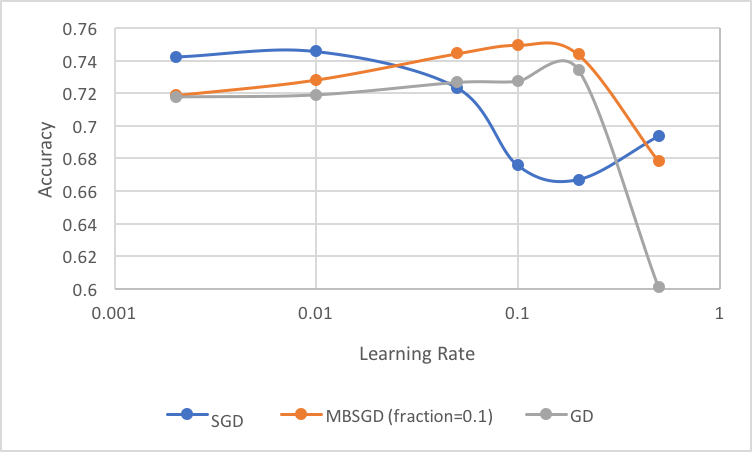
\includegraphics[width=0.48\textwidth]{lr.png}
\caption{Parameter Analysis on Learning Rate}
\label{lr}
\end{figure}

The parameter analysis of regularization coefficient $\lambda$ is shown in Figure \ref{reg}. We run SGD with different regularization coefficients ($\lambda = 0.00001, 0.0001, 0.001, 0.01, 0.05, 0.5$) on the small version of dataset. Other parameters are kept fixed ($\eta$=0, $N$=1). From the result we can see that tuning the regularization coefficient helps little for the final result and large $\lambda$ will harm the performance.

\begin{figure}[t]
\centering
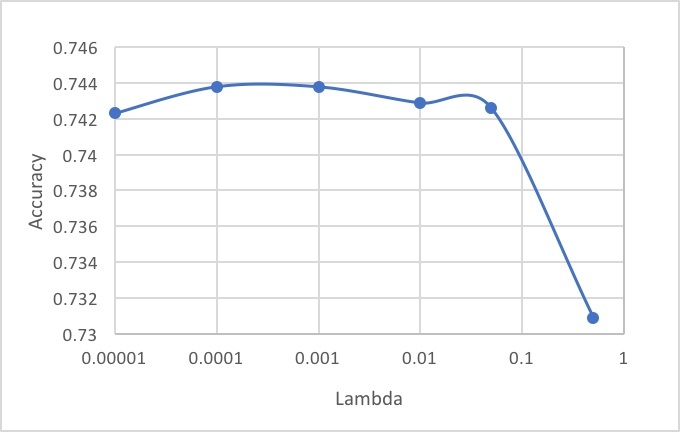
\includegraphics[width=0.48\textwidth]{reg.png}
\caption{Parameter Analysis on Regularization Coefficient}
\label{reg}
\end{figure}

The parameter analysis of epoch $N$ is shown in Figure \ref{reg}. We compare three GD variants with different numbers of epochs ($N = 1, 2, 3, 4$) on the small version of dataset. Other parameters are kept fixed ($\eta$=0, $\lambda$=0.002). From the result we can see that after one epoch, on the other words, after the model goes through the whole dataset for one pass, the performance tends to converge.

\begin{figure}[t]
\centering
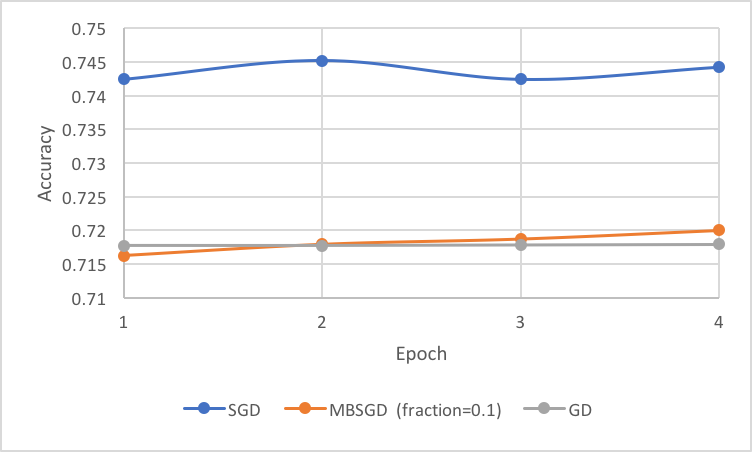
\includegraphics[width=0.48\textwidth]{epoch.png}
\caption{Parameter Analysis on Epoch}
\label{epoch}
\end{figure}

The parameter analysis of batch fraction $f$ is shown in Figure \ref{frac}. We run MBSGD with different fractions ($f = 0.001, 0.01, 0.1, 1$) on the small version of dataset. Other parameters are kept fixed ($\eta = 0$, $\lambda = 0.002$, $N = 3$). From the result we can see that smaller fraction will bring better performance. Note that when $f = 1$, all tweets are sampled for each iteration, which means now MBSGD is essentially the same with GD. Under large fraction setting, the algorithm uses less iterations in one epoch and to achieve same accuracy, epoch number N needs to be larger. 

\begin{figure}[t]
\centering
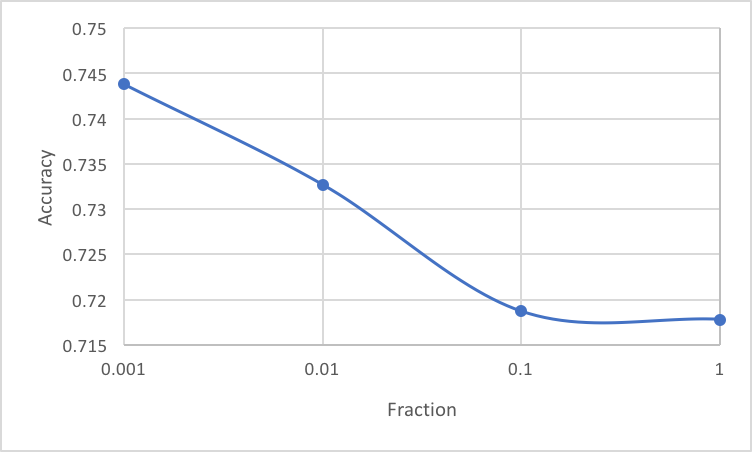
\includegraphics[width=0.48\textwidth]{fraction.png}
\caption{Parameter Analysis on Batch Fraction}
\label{frac}
\end{figure}



\section{Conclusion and Future Work}
\label{sec:conclusionAndFutureWork}

In this project, we summarize our contributions in three points:

\begin{enumerate}  
\item We collect and clean the English stream of tweets text from February 2013 to April 2018 and create the training and test dataset for sentiment analysis with the label infromation from emojis and emoticons.
\item We extract the four byte character feature for each tweet and implement the logistics regression with GD, SGD amd mini-batch SGD for the sentiment analysis on the large scale social media data.
\item We provide the parameter analysis for the three variants of gradient decent on a subset of the whole data.
\end{enumerate}

In the future, we plan to implement more fancy optimization tricks such as momentum, nesterov, learning rate decay and so on. We are also interested in comparing the time efficiency of different variants of gradient decent under the setup of large-scale training data.


% OBLIGATORY: use BIBTEX formatting!
\normalsize

{\vskip 12pt}
\noindent


\bibliographystyle{ACM-Reference-Format}
\bibliography{sample-bibliography}

\end{document}
